\section{Background/Basics}\label{sec:two}
% https://developer.ibm.com/articles/how-cloud-fog-and-mist-computing-can-work-together/#:~:text=Fog%20computing%20takes%20place%20beneath,the%20sensor%20and%20actuator%20devices. %
\subsection{Key Concepts}
\begin{figure}[H]
	\centering
	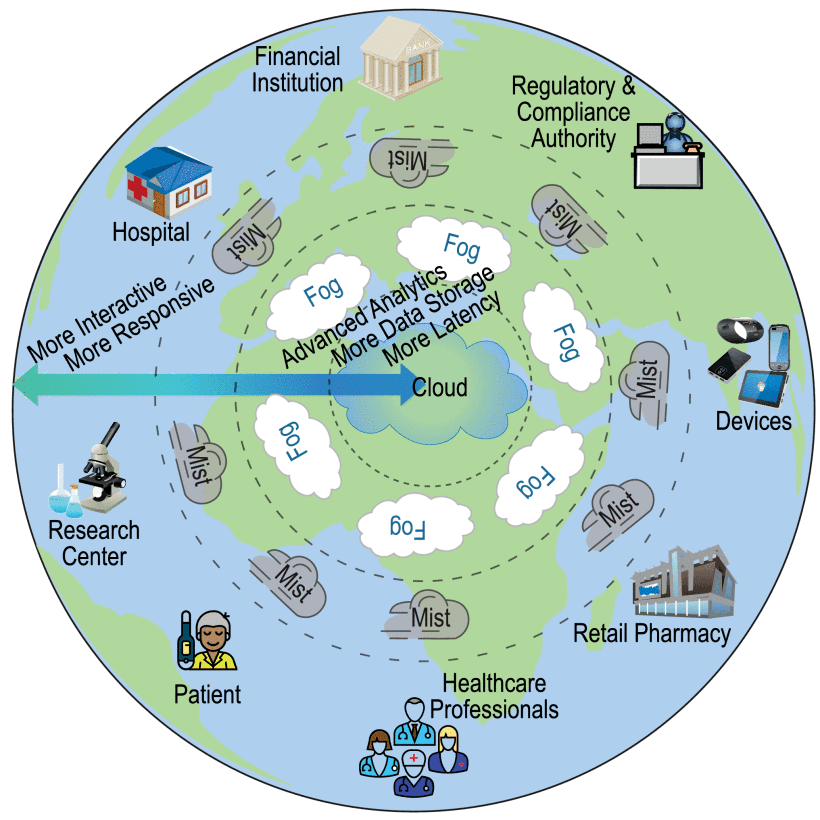
\includegraphics[width=10cm]{image/Fogcloudmist.png}
	\caption{Proposed IoHT Framework with differet stalkholders}
	\caption*{src:ASIF-UR-RAHMAN et al:\cite{3}}
\end{figure}
%https://www.quora.com/What-are-the-functions-of-Cloud-computing-services#:~:text=Cloud%20Computing%20is%20a%20process,software%20services%20using%20internet%20technologies.&text=Web%20Based%20Cloud%20Computing%3A%20Companies,full%20application%20for%20their%20needs. + https://www.quora.com/What-are-the-key-benefits-of-Cloud-computing + https://en.wikipedia.org/wiki/Cloud_computing %
\subsubsection{CLOUD} 
\hfill\\
\hfill\\
Cloud is a centralized mode of computing that can store and access the data and program on the remote servers that are hosted on the internet instead of on the local server or hard-disk.It is also called as Internet based computing because of its main functionalities such as storing,computing,control and communicating between servers on large data centers that are closer to the end user through the cloud-to-things continuum.\\ \\
The main functionality of Cloud services is to help migrate from traditional environment to cloud computing to delivering the services over the internet that can ensure optimized performance,support,consistency and security to the maximum level.\\ \\
The main technology for cloud computing is virtualization which seperates a physical computing device into more than one virtual devices,each performing and managing the computing tasks leading to the agility of increaseed IT operations and reduced cost by making maximum utilization of infrastucture resources.\\ \\
The main aim of cloud computing is to make users utilize the technology and resources to an extent such that they stay focused on their business needs and cut down the cost instead of focusing on other IT related issues such as storage or performance or scalability and etc.\\ \\
Cloud computing shares the same characteristics as like with Fog computing,Grid computing,Client-server model and Peer-to-peer\cite{10}.\\

Cloud consists of three layer of service models based on the services companies provide.\\
\begin{itemize}
	\item Infrastructure as a service(IaaS):\\
	Provision of processing,storage,networks and other fundamental computing resources\cite{mell2011nist}.\\
	\item Platform as a service(PaaS):\\
	Allows for the deployment of customer created applications and these application are restricted to the programming languages,libraries and services supported by the provider.\\
	\item Application/Software as a service(SaaS):\\
	Applications that are running on a cloud infrastructure.Here consumers can use the applications but have no control over the cloud resources such as network,servers,operating systems,storage, technologies or individual applications\cite{mell2011nist}.\\
\end{itemize}
The key characteristics of Cloud Computing are:\\
\begin{itemize}
	\item Scalability: Easy to scale up and scale down according to the business requirements and manage resource utilization instead of installing expensive upgrades.\\
	\item Maintenance and Performance: Maintaining is easy as it can be accessed from any where and ensures performance by frequent upgradation to recent trends leading to fast and efficient computing speed over the web services.\\
	\item Security:Monitoring is one of the main facilities of cloud computing and Data access and security is more efficient through cloud computing than other traditional systems.\\
	\item Resource pooling : Ability to serve multiple clients at a time using the resources that are pooled and this resource usage can be assigned or reassigned based on client needs any time.\\
	\item Broad network access: Enables the capablities of accessing the resources that are hosted in private cloud over the internet through standard mechanisms that promote use by heterogeneous applications such as mobile phones, tablets, laptops, and workstations.
\end{itemize}
\newpage
\subsubsection{FOG}
%from wiki + https://www.geeksforgeeks.org/difference-between-cloud-computing-and-fog-computing/?ref=rp   %
\hfill\\
\hfill\\
Fog Computing is an architecture that extends cloud computing to the edge of the network.It is the concept of a network infrastructure that distributes computation,communication,control and storage closer to the end users along the cloud-to-things continuum\cite{chiang2016fog}.\\ \\
The devices at this layer is responsible for performing operations related to networking such as routers,gateways,bridges and hubs such that it is capable of performing both computational and networking operations simultaneaously.\\ \\
Although the devices in fog layer when compared to cloud are resource constrained ,it ensures a reliable service with geological spread and decentralized nature over a wide area. When compared to the traditional cloud computing,fog computing ensures delay-sensitive service request from the end user with low energy consumption and less traffic congestion\cite{11}.\\ \\
Above all,fog networks are considered as offloading to core computation and storage.Further,the nodes present in the fog network determine whether to process the service using the available resources or send to the cloud server.Hence fog computing helps to attain efficient resource utilization and greater performance concerning the delay,bandwidth and energy consumption\cite{11}.\\ \\
The key characteristics of Fog computing are;\\
\begin{itemize}
	\item Allocates the resources and services to the end users such as computation,communication,control,and storage.\\
	\item Can be fully distributed or mostly centralized or in between.\\
	\item Fog architecture and its applications can be virtualized but can also be implemented in dedicated hardware and software.\\
	\item Allows the same application to run anywhere with reduced need for specific applications just for the cloud,endpoints or edge devices.\\
	\item Allow applications to run on same physical platform without mutual interference from multiple suppliers.\\
	\item Enables the capacity of processing high number of nodes\\
	\item Fog often combines with cloud to allow end-to-end services impeccably.\\
	\item Determines the best way to carry out the computing,storage, and control functions based on the user requirements.\\
	\item Ensures efficiency and performance by pooling the resources anywhere between cloud and end-user systems.\\
	\item Enables a rapid innovation and afforadable scaling which can be much faster and cheaper to experiment with client and edge devices instead of waiting for the vendors of large network and cloud boxes to initiate or adopt innovation.\\
	\item Enables data analytics at the network edge and can support time-sensitive functions for local cyber-physical systems.\\
	
\end{itemize}
\subsubsection{MIST}
%from net(https://radiocrafts.com/cloud-vs-fog-vs-mist-computing-which-one-should-you-use/#:~:text=Mist%20computing%20is%20the%20extreme,of%20micro%2Dcontrollers%20and%20sensors.&text=Enabling%20resource%20harvesting%20by%20computation,monitored%20on%20the%20sensor%20itself.)
\hfill\\
\hfill\\
"Mist computing is an extreme edge of a network consisting of sensors and micro-controllers.Mist computing uses microcomputers and microcontrollers to send to the fog computing nodes and then onwards towards the centralized cloud computing servers.Main functionalities of Mist is to ensure resource collection by computation and communication capabilities to be available and to allow random computations to be provisioned,deployed,managed and monitored on sensors itself\cite{1}".\\ \\
%https://radiocrafts.com/cloud-vs-fog-vs-mist-computing-which-one-should-you-use/#:~:text=Mist%20computing%20is%20the%20extreme,of%20micro%2Dcontrollers%20and%20sensors.&text=Enabling%20resource%20harvesting%20by%20computation,monitored%20on%20the%20sensor%20itself.%
The key characteristics of Mist Computing :\\
\begin{itemize}
	\item In Mist computing the communication takes place at a high speed of computing in an embedded microcontroller which allows to send only relevant data to the gateway,router,or server by collecting the raw data at the edge of your network and then group them by filtering,anomaly identification mechanisms and pattern recognition which helps conserve the battery power as well as bandwidth\cite{1}.\\
	\item Due to the computing power on sensors,it consumes low power for data processing and optimizes the data before storing.\\
	\item All local analytics and decision making happen in mist layer with less overhead.\\
	\item It is highly robust for data and applications.\\
	\item Security is assured as the data is first being processed in the mist layer before sending it to the remote server.\\
	\item By adding mist layer to the existing fog-based architecture it helps in reducing the data volume to be transmitted through IoT devices using rule-based preprocessing of the data\cite{3}.\\
	\item The latency in processing,transmission and computational complexity is reduced by minimal usage of data volume which inturn reduces the power consumption in the framework.\\
	\item Mist facilitates time-critical data processing.\\
	\item Mist remains directly within the network fabric and operates on the extreme edge of the network using sensors and micro controllers\cite{3}.\\
	\item Mist is responsible for performing basic rule-based preprocessing of the the sensor data such as data aggregation,fusion and filtering\cite{3}.\\
\end{itemize}
\newpage
\subsection{SDN-Software Defined Networks}
"Software-Defined Networking is an emerging approach that uses software-based controller or application programming interfaces(APIs) to reconfigure traffic on the network and communicate with the underlying hardware infrastructure\cite{vm}".\\ \\
The main idea of SDN is to seperate physically the control plane and data plane\cite{11}.\\
Due to the increase in the interest of Internet of Things(IoT) and the huge heterogeneous data in the ubiquitous networks,it makes implementation very crucial in network.\\ \\
To maintain these heterogeneous data efficiently by ensuring high QoS in terms of network scalability,privacy and security,the IoT framework relies on Software Defined Networking(SDN)\cite{3} where the network resources are dynamically allocated and deployed on the IoHT technology framework in a centalized/distributed server.\\ \\
SDN helps in fulfilling various requirements of applications and workloads through network virtualization by decoupling control plane from data plane in the IoHT framework to manage the resource demand of increasing IoT devices\cite{3}\cite{haque2016wireless} \\
SDN consists of 3 parts :
\begin{itemize}
	\item Application: Where the resources communicate or request over the internet
	\item Controller: Which is responsible for routing of data packet based on the information collected from application.
	\item Networking devices: Which is responsible for handling and moving of data,based on the request it recieves from the controller.
\end{itemize}
In general,allocating resources,scheduling,routing,flow control,packet-forwarding and other network functionality is handled by the SDN controller(SDNC).These SDN controllers communicate via TCP connection using switches which is responsible for defining fine-grained QoS provisioning based on the attributes and the state of data gathered from fog node\cite{11}.\\  \\
Despite of the fact that Fog is a feasible way for latency-sensitive task\cite{11},the available resources can differ based on the fog computing resources. Hence it is necessary to transfer some of the latency-aware fog tasks to cloud if there is no enough resource in the fog layer\cite{11}.However software defined QoS is provisioned by deploying dynamic QoS policy to handle fog services and SDN benefits from distrbuting latency-aware fog tasks using complete knowledge of network state.\\ \\
SDN not only benefits the network infrastructure by optimizing the flow of data over the internet and prioritize applications availability based on the requirements by customizing the network services and allocating virtual resources in real-time using one centralized location but also ensures robust security by providing visibility to the entire network that can rectify the threat and act accordingly.Different levels of security can be applied at different zones for devices in a large network by the network administrator.\\ \\
SDN plays a major role in edge computing and internet of things because of its speed and flexibility that require transferring of data quickly and easily between remote sites.
%mypaper +https://www.sciencedirect.com/science/article/abs/pii/S1389128618305395%

\newpage
\subsection{Cloud Features}
"Cloud computing is a model for enabling ubiquitous,convenient,on demand network access to a shared pool of configurable computer resources that can be rapidly provisioned and released with minimal management effort or service provider interaction\cite{mell2011nist}"\\

Main objective is to compile,store,interconnect and manage on demand that supports various operating systems,programming languages,tools,databases and devices.[from Mobicom-KTR-Slides] \\ \\
Which implies,
\begin{itemize}
	\item Having scalability in distributed computing utilizing resource pools
	\item Storing large amount data(terabytes)
	\item Making a gateway for connections between applications to servers through IP networks
	\item Utlizing the scaling and multiplexing effects of resource usage
\end{itemize}
Example : Microsoft Azure studies\\ \\
"Microsoft stands as one among the five Cloud market leaders that provide Infrastructure as a service [IaaS], Platform-as-a-Service[PaaS] and Software-as-a-Service [SaaS]\cite{azure}"\\ \\
Comman characteristics are,\\
\begin{itemize}
	\item Application management:\\
	Easy to build,deploy and manage apps by customizing cloud software.\\
	\item Flexibility:\\
	Flexibile in choosing the functionalities according to the business infrastructure.\\
	\item Agility:\\
	Fast and up-to-date in terms of deploy,operation and scalability making infrastructure and applications agile.\\
	\item Compliance:\\
	Security and privacy demands ensured in maintaing the data stored.\\
	\item Storage:\\
	Faster and reliable delivery rate in terms of sharing data across the virtual machines by facilititaing optimal user experience and store heterogeneous data.\\
	\item Security:\\
	Security being highly ensured by having two-tier authentication protocol using hand biometric readers,proxy card access readers and etc.
	
	%https://www.mercurysolutions.co/blog/top-11-business-benefits-of-microsoft-azure%
\end{itemize}
